\documentclass{standalone}
\usepackage{tikz}
\usetikzlibrary{patterns, positioning}

\begin{document}
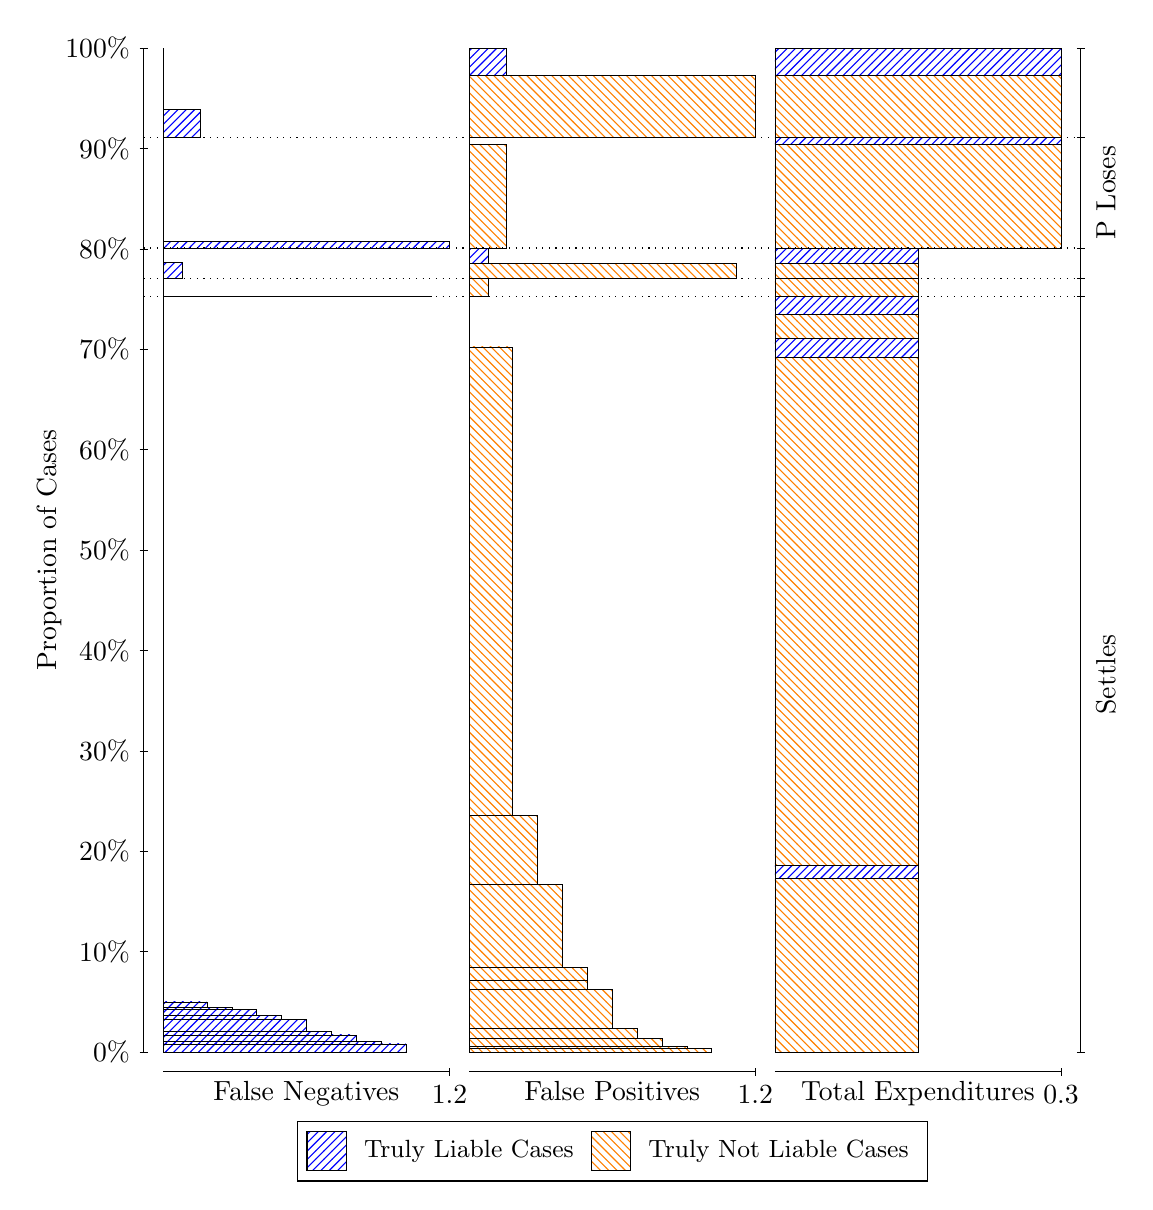
\begin{tikzpicture}
\draw[black, very thin] (1.5,1.75) -- (1.5,14.5);
\node[rotate=90, anchor=center] at (0.3, 8.125) {Proportion of Cases};
\draw[black, very thin] (1.45,1.75) -- (1.55,1.75);
\node[anchor=east] at (1.45, 1.75) {0\%};
\draw[black, very thin] (1.45,3.025) -- (1.55,3.025);
\node[anchor=east] at (1.45, 3.025) {10\%};
\draw[black, very thin] (1.45,4.3) -- (1.55,4.3);
\node[anchor=east] at (1.45, 4.3) {20\%};
\draw[black, very thin] (1.45,5.575) -- (1.55,5.575);
\node[anchor=east] at (1.45, 5.575) {30\%};
\draw[black, very thin] (1.45,6.85) -- (1.55,6.85);
\node[anchor=east] at (1.45, 6.85) {40\%};
\draw[black, very thin] (1.45,8.125) -- (1.55,8.125);
\node[anchor=east] at (1.45, 8.125) {50\%};
\draw[black, very thin] (1.45,9.4) -- (1.55,9.4);
\node[anchor=east] at (1.45, 9.4) {60\%};
\draw[black, very thin] (1.45,10.675) -- (1.55,10.675);
\node[anchor=east] at (1.45, 10.675) {70\%};
\draw[black, very thin] (1.45,11.95) -- (1.55,11.95);
\node[anchor=east] at (1.45, 11.95) {80\%};
\draw[black, very thin] (1.45,13.225) -- (1.55,13.225);
\node[anchor=east] at (1.45, 13.225) {90\%};
\draw[black, very thin] (1.45,14.5) -- (1.55,14.5);
\node[anchor=east] at (1.45, 14.5) {100\%};

\draw[black, very thin] (13.4,1.75) -- (13.4,14.5);
\draw[black, very thin] (13.35,1.75) -- (13.45,1.75);
\node[anchor=west] at (13.35, 1.75) {};
\draw[black, very thin] (13.35,11.341) -- (13.45,11.341);
\node[anchor=west] at (13.35, 11.341) {};
\draw[black, very thin] (13.35,11.574) -- (13.45,11.574);
\node[anchor=west] at (13.35, 11.574) {};
\draw[black, very thin] (13.35,11.96) -- (13.45,11.96);
\node[anchor=west] at (13.35, 11.96) {};
\draw[black, very thin] (13.35,13.367) -- (13.45,13.367);
\node[anchor=west] at (13.35, 13.367) {};
\draw[black, very thin] (13.35,14.5) -- (13.45,14.5);
\node[anchor=west] at (13.35, 14.5) {};

\draw[black, very thin, pattern color=blue, pattern=north east lines] (1.75,1.75) rectangle (4.8304,1.8534);
\draw[black, very thin, pattern color=blue, pattern=north east lines] (1.75,1.8534) rectangle (4.5145,1.8854);
\draw[black, very thin, pattern color=blue, pattern=north east lines] (1.75,1.8854) rectangle (4.1986,1.9676);
\draw[black, very thin, pattern color=blue, pattern=north east lines] (1.75,1.9676) rectangle (3.8826,2.0127);
\draw[black, very thin, pattern color=blue, pattern=north east lines] (1.75,2.0127) rectangle (3.5667,2.1596);
\draw[black, very thin, pattern color=blue, pattern=north east lines] (1.75,2.1596) rectangle (3.2507,2.2131);
\draw[black, very thin, pattern color=blue, pattern=north east lines] (1.75,2.2131) rectangle (2.9348,2.2873);
\draw[black, very thin, pattern color=blue, pattern=north east lines] (1.75,2.2873) rectangle (2.6188,2.3193);
\draw[black, very thin, pattern color=blue, pattern=north east lines] (1.75,2.3193) rectangle (2.3029,2.3869);
\draw[black, very thin, pattern color=orange, pattern=north west lines] (1.75,2.3869) rectangle (1.75,11.341);
\draw[black, very thin, pattern color=blue, pattern=north east lines] (1.75,11.341) rectangle (5.1464,11.345);
\draw[black, very thin, pattern color=orange, pattern=north west lines] (1.75,11.345) rectangle (1.75,11.574);
\draw[black, very thin, pattern color=blue, pattern=north east lines] (1.75,11.574) rectangle (1.987,11.773);
\draw[black, very thin, pattern color=orange, pattern=north west lines] (1.75,11.773) rectangle (1.75,11.96);
\draw[black, very thin, pattern color=blue, pattern=north east lines] (1.75,11.96) rectangle (5.3833,12.046);
\draw[black, very thin, pattern color=orange, pattern=north west lines] (1.75,12.046) rectangle (1.75,13.367);
\draw[black, very thin, pattern color=blue, pattern=north east lines] (1.75,13.367) rectangle (2.2239,13.717);
\draw[black, very thin, pattern color=orange, pattern=north west lines] (1.75,13.717) rectangle (1.75,14.5);
\draw[black, very thin, pattern color=orange, pattern=north west lines] (5.6333,1.75) rectangle (8.7138,1.7962);
\draw[black, very thin, pattern color=orange, pattern=north west lines] (5.6333,1.7962) rectangle (8.3978,1.8241);
\draw[black, very thin, pattern color=orange, pattern=north west lines] (5.6333,1.8241) rectangle (8.0819,1.9239);
\draw[black, very thin, pattern color=orange, pattern=north west lines] (5.6333,1.9239) rectangle (7.7659,2.0464);
\draw[black, very thin, pattern color=orange, pattern=north west lines] (5.6333,2.0464) rectangle (7.45,2.544);
\draw[black, very thin, pattern color=orange, pattern=north west lines] (5.6333,2.544) rectangle (7.1341,2.6668);
\draw[black, very thin, pattern color=orange, pattern=north west lines] (5.6333,2.6668) rectangle (7.1341,2.8289);
\draw[black, very thin, pattern color=orange, pattern=north west lines] (5.6333,2.8289) rectangle (6.8181,3.8795);
\draw[black, very thin, pattern color=orange, pattern=north west lines] (5.6333,3.8795) rectangle (6.5022,4.7507);
\draw[black, very thin, pattern color=orange, pattern=north west lines] (5.6333,4.7507) rectangle (6.1862,10.704);
\draw[black, very thin, pattern color=blue, pattern=north east lines] (5.6333,10.704) rectangle (5.6333,11.341);
\draw[black, very thin, pattern color=orange, pattern=north west lines] (5.6333,11.341) rectangle (5.8703,11.57);
\draw[black, very thin, pattern color=blue, pattern=north east lines] (5.6333,11.57) rectangle (5.6333,11.574);
\draw[black, very thin, pattern color=orange, pattern=north west lines] (5.6333,11.574) rectangle (9.0297,11.762);
\draw[black, very thin, pattern color=blue, pattern=north east lines] (5.6333,11.762) rectangle (5.8703,11.96);
\draw[black, very thin, pattern color=orange, pattern=north west lines] (5.6333,11.96) rectangle (6.1072,13.281);
\draw[black, very thin, pattern color=blue, pattern=north east lines] (5.6333,13.281) rectangle (5.6333,13.367);
\draw[black, very thin, pattern color=orange, pattern=north west lines] (5.6333,13.367) rectangle (9.2667,14.151);
\draw[black, very thin, pattern color=blue, pattern=north east lines] (5.6333,14.151) rectangle (6.1072,14.5);
\draw[black, very thin, pattern color=orange, pattern=north west lines] (9.5167,1.75) rectangle (11.333,3.9567);
\draw[black, very thin, pattern color=blue, pattern=north east lines] (9.5167,3.9567) rectangle (11.333,4.116);
\draw[black, very thin, pattern color=orange, pattern=north west lines] (9.5167,4.116) rectangle (11.333,10.567);
\draw[black, very thin, pattern color=blue, pattern=north east lines] (9.5167,10.567) rectangle (11.333,10.817);
\draw[black, very thin, pattern color=orange, pattern=north west lines] (9.5167,10.817) rectangle (11.333,11.114);
\draw[black, very thin, pattern color=blue, pattern=north east lines] (9.5167,11.114) rectangle (11.333,11.341);
\draw[black, very thin, pattern color=orange, pattern=north west lines] (9.5167,11.341) rectangle (11.333,11.57);
\draw[black, very thin, pattern color=blue, pattern=north east lines] (9.5167,11.57) rectangle (11.333,11.574);
\draw[black, very thin, pattern color=orange, pattern=north west lines] (9.5167,11.574) rectangle (11.333,11.762);
\draw[black, very thin, pattern color=blue, pattern=north east lines] (9.5167,11.762) rectangle (11.333,11.96);
\draw[black, very thin, pattern color=orange, pattern=north west lines] (9.5167,11.96) rectangle (13.15,13.281);
\draw[black, very thin, pattern color=blue, pattern=north east lines] (9.5167,13.281) rectangle (13.15,13.367);
\draw[black, very thin, pattern color=orange, pattern=north west lines] (9.5167,13.367) rectangle (13.15,14.151);
\draw[black, very thin, pattern color=blue, pattern=north east lines] (9.5167,14.151) rectangle (13.15,14.5);
\draw[black, dotted] (1.5,11.341) -- (13.4,11.341);
\draw[black, dotted] (1.5,11.574) -- (13.4,11.574);
\draw[black, dotted] (1.5,11.96) -- (13.4,11.96);
\draw[black, dotted] (1.5,13.367) -- (13.4,13.367);
\draw[black, very thin] (1.75,1.5) -- (5.3833,1.5);
\node[anchor=north] at (3.5667, 1.5) {False Negatives};
\draw[black, very thin] (5.3833,1.45) -- (5.3833,1.55);
\node[anchor=north] at (5.3833, 1.45) {1.2};

\draw[black, very thin] (5.6333,1.5) -- (9.2667,1.5);
\node[anchor=north] at (7.45, 1.5) {False Positives};
\draw[black, very thin] (9.2667,1.45) -- (9.2667,1.55);
\node[anchor=north] at (9.2667, 1.45) {1.2};

\draw[black, very thin] (9.5167,1.5) -- (13.15,1.5);
\node[anchor=north] at (11.333, 1.5) {Total Expenditures};
\draw[black, very thin] (13.15,1.45) -- (13.15,1.55);
\node[anchor=north] at (13.15, 1.45) {0.3};

\node[black, centered, rotate=90] at (13.72, 6.5455) {Settles};


\node[black, centered, rotate=90] at (13.72, 12.664) {P Loses};


\draw (7.449999999999999,1.5) node[draw=none] (baseCoordinate) {};
\begin{scope}[align=center]
        \matrix[scale=0.5, draw=black, below=0.5cm of baseCoordinate, nodes={draw}, column sep=0.1cm]{
            \node[rectangle, draw, minimum width=0.5cm, minimum height=0.5cm, pattern=north east lines, pattern color=blue] {}; &
            \node[draw=none, font=\small] (B) {Truly Liable Cases}; &
            \node[rectangle, draw, minimum width=0.5cm, minimum height=0.5cm, pattern=north west lines, pattern color=orange] {}; &
            \node[draw=none, font=\small] (B) {Truly Not Liable Cases}; \\
            };
\end{scope}

\end{tikzpicture}
\end{document}